\documentclass[11pt]{article}
\usepackage[a4paper,margin=1in]{geometry}
\usepackage[T1]{fontenc}
\usepackage{lmodern}
\usepackage{microtype}
\usepackage{amsmath,amssymb}
\usepackage{graphicx}
\usepackage{booktabs}
\usepackage{multirow}
\usepackage[table]{xcolor}
\usepackage{enumitem}
\usepackage{caption}
\usepackage[numbers,sort&compress]{natbib}
\usepackage[colorlinks=true,linkcolor=blue!50!black,citecolor=blue!50!black,urlcolor=blue!50!black]{hyperref}
\usepackage[capitalise,noabbrev]{cleveref}
\usepackage{listings}
\lstset{basicstyle=\ttfamily\footnotesize,breaklines=true,columns=fullflexible,frame=single,framerule=0.3pt}
\setlist{nosep,leftmargin=*}
\newcommand{\tauw}{\tau}
\newcommand{\KH}{KH-1}

\title{Write Where Short Memory Cannot Reach:\\Distance-Invariant Fact Recall in Fixed-State Language Models}
\author{Youssef Khouidi\\01TEK LLC\\\texttt{ucefkh@01tek.com}}
\date{October 2026\\[2pt]\small DOI: \href{https://doi.org/10.5281/zenodo.23447665}{10.5281/zenodo.23447665}}

\begin{document}
\maketitle

\begin{abstract}
Fixed-state recurrent language models such as Gated DeltaNet and Mamba promise constant memory at any context length, yet in practice they recall a fact a few thousand tokens later and then lose it. We separate the two ways a delta-rule memory forgets, \emph{decay} and \emph{erasure by later writes}, and remove both on dedicated \emph{archival heads} whose decay is pinned to one and whose writes must pass a hard threshold. On synthetic streams this gives distance-invariant recall: 2.2M-parameter models trained on 256-token sequences recall up to 32 facts after 1M tokens in 9/9 seeds. For language models the architecture is necessary but not sufficient. With truncated backpropagation, writes are learned only from queries inside the same segment, and if a bounded-memory layer can answer those queries, recall is routed through that layer and ends at its horizon. Making in-segment queries unanswerable by bounded memory, the \emph{routing principle}, yields 117M-parameter models whose recall of facts spliced into FineWeb-Edu text is flat from 16K to 1M tokens in all six runs with a short non-archival half-life, and a 494M model at 0.88 at 1M. The same principle lets us graft the memory onto frozen pretrained models as small adapters: the base model runs on bounded chunks, and the adapters learn to carry facts across them. With a write-threshold curriculum (train one step below the inference threshold), the released LFM2-350M graft recalls 0.90 of facts read 1M tokens earlier on fresh evaluation streams, in 0.84\,GB of GPU memory, and a Qwen3.5-4B graft also 0.90. The curriculum raises 1M recall in all three training seeds we ran, but the level varies across seeds (0.575--0.95). Carrying the memory across chunks also lowers perplexity by 2--5\%. After short single-GPU runs the graft also transfers to a mixture-of-experts base (LFM2.5-8B-A1B, 0.35--0.375 at 1M) and to an attention-only base (Gemma 4 E2B, flat from 16K to 1M at 0.40--0.575). On BABILong, a short adapter fine-tune of the 350M graft gives 0.50--0.61 from 0K to 1M, two to three times a retrieval baseline from 4K up. We document four training-signal traps that silently produce models which fail on fresh facts or never learn long-range recall, and release code, adapters and all evaluation logs.
\end{abstract}

\section{Introduction}
\label{sec:intro}
Attention keeps every past token in a key--value cache, so its memory grows linearly with context. Fixed-state sequence models (linear attention and its delta-rule variants \citep{schlag2021,deltanet2024,gdn2024}, selective state-space models \citep{mamba2023,mamba2_2024,mamba3_2025} and modern RNNs \citep{rwkv7_2025}) instead compress the past into a state of constant size. That makes them attractive for unbounded streams, but exact recall is their known weakness: a fixed state cannot store an unbounded number of tokens, and recall-intensive tasks expose the gap to attention \citep{jelassi2024,zoology2023,based2024}.

We study a narrower question that matters in practice: can a fixed-state model recall a \emph{small number} of facts, read once, after a \emph{long and arbitrary} stretch of ordinary text? Here capacity is not the binding constraint. A few facts fit easily in a state of thousands of dimensions, yet the Gated DeltaNet and Mamba-3 models we trained recalled them to about sixteen times their training length and then lost them (\cref{sec:synthetic}). The failure comes from \emph{how} the state is written and from \emph{what the training signal teaches it to write}.

A delta-rule memory forgets in two ways. \emph{Decay} shrinks the whole state at every step; \emph{erasure} happens when a later write uses a key that overlaps the stored fact's key and overwrites part of it. We remove decay on a few \emph{archival heads} by pinning their decay to one, force every other head to forget, and make archival writes sparse with a hard write threshold. On synthetic streams this is enough for distance-invariant recall. On language models it is not. Trained with truncated backpropagation through time (TBPTT) \citep{tbptt1990}, a write receives gradient only from queries in its own segment. If a bounded-memory layer can satisfy those queries, the network routes facts through it, and recall stops at that layer's horizon. Whether a run extrapolates then becomes a seed lottery. We call the fix the \emph{routing principle}: make in-segment queries hard or impossible to answer with bounded memory, so that the archival heads earn the gradient.

The principle also gives a cheap way to add the memory to existing models. Running a frozen pretrained model on bounded chunks makes it a bounded-memory layer by construction. Small archival adapters inserted between its blocks are then the only path across chunks, and they learn to carry facts there. We call the resulting models \KH{}.

\paragraph{Contributions.}
\begin{enumerate}
\item \textbf{Mechanism.} We separate decay from erasure, with an exact kernel-level retention measure, and show that removing both on archival heads gives distance-invariant recall on synthetic streams; at 64K tokens, capacity is set by the archival key dimension (\cref{sec:background,sec:synthetic}).
\item \textbf{The routing principle.} A fixed-state language model extrapolates recall reliably only when its in-segment training signal is hard to satisfy with its bounded-memory layers. With far-gap drills and a short half-life on non-archival layers, all six such runs of a 117M model are flat from 16K to 1M tokens, and a 494M model reaches 0.88 at 1M (\cref{sec:lm}).
\item \textbf{Training-signal traps.} Four failure modes, each of which looked like an architectural failure: fact recurrence (weight memorisation), memory overload, a collapse of long-range training recall, and state resets from gradient-spike guards (\cref{sec:traps}).
\item \textbf{Grafting onto frozen models.} Archival adapters on frozen LFM2 \citep{lfm2} and Qwen3.5 \citep{qwen35} models, a write-threshold curriculum that raises 1M-token recall in every training seed we ran, write-statistics diagnostics that explain what the gate learns, controls showing that the memory costs no language-modelling quality, and fresh-stream and multi-seed checks of the headline numbers (\cref{sec:graft}).
\item \textbf{Practical notes.} Kernel-correctness traps on Hopper and Blackwell GPUs, evaluation pitfalls, a faster training path checked against the reference implementation, and a full reproducibility appendix with every training command (\cref{app:kernels,app:engineering,app:pitfalls,app:repro}).
\end{enumerate}

\section{Background: decay versus erasure}
\label{sec:background}
A gated delta-rule layer \citep{schlag2021,deltanet2024,gdn2024} keeps a matrix state per head,
\begin{equation}
S_t = \alpha_t\, S_{t-1}\bigl(I - \beta_t k_t k_t^{\top}\bigr) + \beta_t\, v_t k_t^{\top}, \qquad o_t = S_t\, q_t ,
\end{equation}
with unit-norm keys $k_t$, a decay $\alpha_t\in(0,1]$ and a write strength $\beta_t\in[0,1]$. A fact $(k_f, v_f)$ written at time $0$ and read with $q = k_f$ after $D$ further tokens returns $v_f\, k_f^{\top} M_D\, k_f$ plus crosstalk, with $M_D = \prod_{t=1}^{D} \alpha_t (I - \beta_t k_t k_t^{\top})$. We call $r_D = k_f^{\top} M_D k_f$ the \emph{retention} of the fact and compute it exactly with the training kernel itself.

\begin{itemize}
\item \textbf{Decay.} $\prod_t \alpha_t \to 0$ unless $\alpha \equiv 1$ on the heads that hold facts.
\item \textbf{Erasure.} Every later write removes the component of the stored key along its own key. For isotropic keys, $\log \mathbb{E}[r_D] \approx -\sum_t \beta_t / d_k$. Distance invariance therefore needs $\beta_t \to 0$ on everything except facts, or writes confined to a subspace orthogonal to the fact keys.
\end{itemize}

\section{Method}
\label{sec:method}
\subsection{Archival delta memory}
\label{sec:hais}
Our memory layer (\texttt{hais}) is a gated delta-rule layer built on the \texttt{flash-linear-attention} kernels \citep{fla} with L2-normalised queries and keys, short causal convolutions and an output gate. Of its $H$ heads, $A$ are \emph{archival}: their log-decay is pinned to $0$, so they never forget on their own. Three further choices make archival memory stable on unbounded streams.
\begin{itemize}
\item \textbf{Forced forgetting} for non-archival heads: their log-decay is clamped to $\le -0.35$ per token. The decay must \emph{underflow} within the training window, because an RMS-normalised read is invariant to a uniform shrinkage of the state (\cref{sec:synth_recipe}).
\item \textbf{Sparse archival writes.} A hard write threshold $\tauw$: archival writes with $\beta \le \tauw$ are exactly zero in the forward pass, with a straight-through gradient \citep{ste2013}. In language models we add an L1 penalty on archival $\beta$ at ordinary-text tokens only; inserted facts and queries are not penalised.
\item \textbf{Value normalisation.} $v \leftarrow s\, v / \lVert v\rVert$. For spread-out keys this keeps $\lVert S\rVert_F$ near $\sqrt{d_k}\, s$ (a typical level, not a worst-case bound), so the state does not drift on unbounded streams.
\end{itemize}
In language models built from scratch, archival layers alternate with Gated DeltaNet (GDN) layers \citep{gdn2024}, whose log-decay we clamp to $\le -\ln 2 / h$, a half-life of $h$ tokens, so that only archival heads carry long-range state.

\subsection{Language-model training}
\label{sec:lm_training}
Each batch row is a \emph{lane} of continuous FineWeb-Edu text \citep{fineweb2024} whose recurrent state is carried across all training steps (TBPTT with 1{,}024-token segments; 2{,}048 for the 494M model). Facts are spliced into the text from sentence templates with random names and values. Each fact is asked once and never restated, and no two live facts in a lane share a name (\cref{sec:traps}); names themselves recur across training, since the syllable vocabulary yields 14{,}400 of them. Two kinds of queries supervise the memory: \emph{drill lanes} hold 8 facts and their queries inside one segment, and \emph{long-range queries} ask each fact once at a log-uniform age. The mean loss over answer tokens is added with weight 5, which upweights each answer token by about three orders of magnitude relative to a text token. With \emph{far drills}, facts sit in the first 15\% of a segment and their queries in the last 15\%, so drill gaps are at least about 530 tokens (median about 780; standard drills have a median gap of about 510).

\subsection{Grafting onto a frozen model}
\label{sec:graft_method}
To add the memory to a pretrained model we freeze it and run it \emph{chunk-locally}: its attention, convolutions and (for Qwen3.5) Gated DeltaNet layers see one chunk of $C$ tokens at a time, with no key--value cache and no recurrent state carried across chunks. For LFM2 every chunk starts with the model's BOS token: on 1{,}024-token FineWeb-Edu chunks, LFM2-350M's loss is 3.06 with it and 5.16 without. Three archival adapters are inserted between blocks (after LFM2 blocks 7, 11 and 15; after Qwen3.5 layers 15, 23 and 31). Every adapter head is archival, values are normalised, and the adapter output enters the residual stream through a ReZero gate initialised at zero \citep{rezero2020}, so training starts from exactly the base model. Only the adapters are trained, in the spirit of adapter tuning \citep{adapters2019}.

\paragraph{Routing by construction.} Training segments are two chunks long. Drill facts appear in the first chunk and are queried in the second, which the base model cannot see across, so the adapters are the only path that can earn the gradient. This is the routing principle with no extra mechanism.

\paragraph{Data and losses.} Facts use 358 phrasings: 318 compositional ones (6 sentence frames $\times$ 53 attributes) and 40 sentence templates. Half of the queries are rendered as chat turns with the model's chat template. The language-modelling loss is computed on a random 10\% of positions, to keep the frozen model's behaviour, together with every answer position. An L1 penalty on archival writes at non-fact tokens keeps the memory for facts.

\paragraph{Write-threshold curriculum.} A fresh adapter writes with $\beta \approx 0.12$ (its write bias starts at $-2$), so a threshold of 0.9 would zero every write and no gradient would reach the memory. We therefore train in stages: $\tauw = 0.5$, then fine-tunes at $\tauw = 0.9$ and, for LFM2, $\tauw = 0.97$, and we run each model at inference with a threshold one step above its last training threshold (\cref{sec:curriculum}).

\subsection{Streaming evaluation}
\label{sec:eval}
All evaluation is streaming: a chunked forward pass with the state carried across chunks, which uses $O(1)$ memory at any length and matches a full forward pass to numerical precision (\texttt{poc\_m3/smoke.py}). For each cell we splice $K$ fresh facts into the first 10\% of a window of $L$ validation tokens and query them at the end, so every fact is at least $0.9L$ tokens old. A fact counts only if every answer token is the argmax prediction. With $K = 1$ each cell averages 40 independent streams; with $K = 8$, 20 streams of 8 facts. The stream sampler is seeded identically for every model. ``Trained phrasings'' use the training templates with fresh names and values; ``unseen phrasings'' combine sentence frames and attributes that never occur in training; ``chat'' renders the question as a chat turn.

\section{Synthetic results}
\label{sec:synthetic}
\paragraph{Task.} Zipf-distributed filler tokens carry $K$ facts \texttt{[FACT k v]} and end with a query block; only the query positions are supervised, and keys are fresh in every sequence. Facts sit in the first 5\% of the stream (early mode) or anywhere (uniform mode); a decoy variant replaces 10\% of positions with random key and value tokens. Training sequences are 256 tokens long; the recurrent state is passed on to the next batch with probability 0.95 (about 20 batches, or 5K tokens, on average), while training fact--query distances stay within 256 tokens. At 1M tokens each seed is evaluated on 16 streams for $K = 1$ and 2 streams for $K = 8$ and $K = 32$.

\paragraph{Models without archival heads lose facts beyond a few thousand tokens.} Gated DeltaNet trained at 256 tokens recalls perfectly to 4K tokens and is near zero by 64K (\cref{fig:synthetic}). Mamba-3 recalls a single fact to 4K but is weak at $K \ge 8$ even at 256 tokens; one of three Mamba-3 seeds with long-chain state passing holds $K = 1$ to 1M while $K = 8$ stays near 0.33. Attention was evaluated only to 4K.

\begin{figure}[t]
\centering
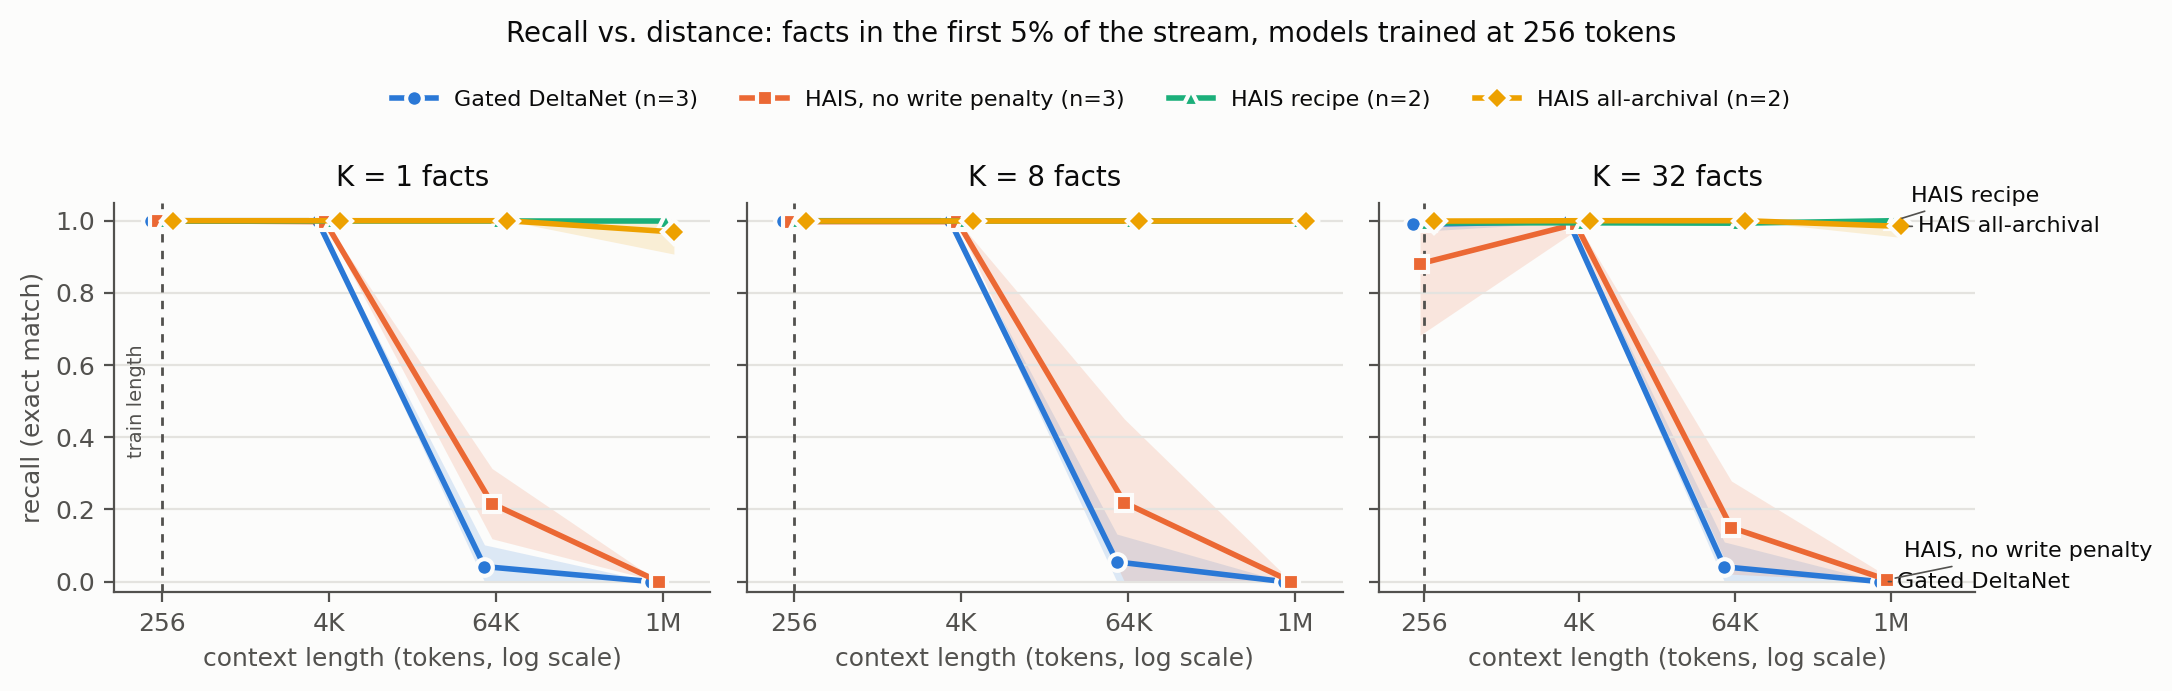
\includegraphics[width=\linewidth]{fig_recall_vs_length.png}
\caption{Synthetic recall versus distance for models trained at 256 tokens, with facts in the first 5\% of the stream. Gated DeltaNet and an archival model without the write penalty collapse beyond 4K tokens; the archival recipe stays at 1.00 to 1M tokens for $K = 1, 8, 32$ facts. Shaded bands span seeds.}
\label{fig:synthetic}
\end{figure}

\subsection{The recipe, and why each part is needed}
\label{sec:synth_recipe}
\Cref{tab:synth_recipe} adds the parts of the recipe one at a time. Archival heads alone extrapolate in only one of three seeds. A weak forced forgetting (a 32-token half-life) is not enough: the escaping seeds collapse by about 4K tokens, which matches fp32 underflow of a non-archival head decaying at the floor ($2^{-126}$ after about 4K tokens). This is consistent with the facts being held in a non-archival head whose shrinkage the RMS-normalised read hides; the key analysis that attributed them to such a head was not archived. Forced forgetting strong enough to underflow within the training window removes this escape route.

\begin{table}[t]
\centering
\caption{Synthetic recipe ablation: seeds with recall $\ge 0.98$ at 1M tokens for every $K \in \{1, 8, 32\}$ (per seed: 16 streams for $K = 1$, 2 streams for $K = 8, 32$).}
\label{tab:synth_recipe}
\resizebox{\linewidth}{!}{\begin{tabular}{@{}lc@{}}
\toprule
Variant & Seeds $\ge 0.98$ at 1M \\
\midrule
archival heads + archival L1 0.05, no forced forgetting & 1/3 \\
+ forced forgetting at a 32-token half-life & 3/6 \\
+ forced forgetting at 0.35 per token, 20K steps & 8/12 \\
\textbf{+ 40K steps (final recipe)} & \textbf{9/9}: mean 1.00 / 1.00 / 0.997 for $K = 1/8/32$ \\
+ hard threshold $\tauw = 0.1$ & 3/3: 1.00 / 1.00 / 1.00 \\
\bottomrule
\end{tabular}}
\end{table}

\subsection{Capacity is set by the archival key dimension}
At 64K tokens, recall falls with the number of stored facts at a rate set by the archival key dimensions (\cref{tab:capacity}). At 1M tokens, large-$K$ recall still decays in most seeds: after 40K training steps, $K = 128$ recall is 0.56 on average (one of four seeds is flat). With twice the training, two of three seeds are flat, and the best holds 0.98 / 0.97 / 0.81 at \emph{1M} tokens for $K = 128 / 256 / 512$.

\begin{table}[t]
\centering
\caption{Synthetic capacity: recall at 64K tokens (mean $\pm$ 1.96 standard errors over 4 seeds).}
\label{tab:capacity}
\begin{tabular}{@{}lccc@{}}
\toprule
Archival capacity & $K = 128$ & $K = 256$ & $K = 512$ \\
\midrule
4 heads $\times$ 64 dims & 0.96 $\pm$ 0.05 & 0.74 $\pm$ 0.12 & 0.34 $\pm$ 0.13 \\
8 heads $\times$ 64 dims & 0.99 $\pm$ 0.01 & 0.87 $\pm$ 0.04 & 0.49 $\pm$ 0.06 \\
\bottomrule
\end{tabular}
\end{table}

\paragraph{Decoys remain open.} With random key and value tokens at 10\% of positions, recall is at least 0.94 to 64K tokens. At 1M it depends on training: models trained with 30\% decoys average about 0.6 (the best seeds 1.00), while models trained with 10\% decoys average 0.00--0.54 across ten configurations. A mis-gated decoy is a full-strength overwrite, about 100 hits per key over 1M tokens.

\section{Language models trained from scratch}
\label{sec:lm}
\paragraph{Setup.} FineWeb-Edu with the GPT-2 tokenizer. The 117M model has $d = 768$ and 12 blocks alternating \texttt{gdn} and \texttt{hais} layers, with 6 of 12 heads archival in each \texttt{hais} layer, trained on 1B tokens; the 494M model has $d = 1536$ and 16 blocks. The baseline is a 12-layer Gated DeltaNet trained identically. Unless stated otherwise, inference uses an archival write threshold of 0.9 and recall is reported as $K = 1$ / $K = 8$.

\paragraph{Necessary ingredients.} Value normalisation is required: in an earlier 49M model without it (and with an archival write penalty), one layer's state norm grew from 207 to 9{,}772 over a 2M-token carried stream, the loss rose from 4.27 to 7.32, and validation perplexity reached 1{,}403. Archival layers alone do not cost perplexity (41.5 versus 42.9 for a matched GDN in an early 117M run; 52.2 versus 56.8 on the final data), although the full recall recipe raises it (53.6--62.6 for the far-drill runs). On real text, erasure is dominated by weak writes: dropping archival writes with $\beta \le 0.9$ at inference lifts 1M-token recall from 0 to 0.38 (19 of 50 streams) without retraining.

\subsection{The levers, and the seed lottery}
\label{sec:levers}
\Cref{tab:levers} combines three training levers: the write threshold, the GDN half-life cap and the text-write penalty. The text-write penalty is necessary, and the GDN cap makes recall flat; with all three, three seeds reach 0.825--0.975 at 1M. Yet with standard drills, extrapolation is fragile. Seed 5 of the same recipe fails, and so do several single-seed variants (learning rate $6\cdot10^{-4}$, drill fraction 0.15, 40 phrasings) and the 494M model; these variants, and a failed seed 3, also ran with a gradient-spike guard that reset the state on 5--291 steps (trap~4), so they are confounded. With compositional facts, only 1 of 10 runs reached 0.90 at 1M, and the same setting with two further seeds reached 0.125 and 0.20.

\begin{table}[t]
\centering
\caption{117M models with standard (half-gap) drills, recall $K = 1$ / $K = 8$ at inference threshold 0.9 ($K = 1$: 40 streams; $K = 8$: 20 streams of 8 facts). The ``$\tauw$ + cap'' row spans two seeds.}
\label{tab:levers}
\resizebox{\linewidth}{!}{\begin{tabular}{@{}lccc@{}}
\toprule
Training levers & 16K & 131K & 1M \\
\midrule
\texttt{gdn} baseline & 0.05 / 0.03 & 0.08 / 0.05 & 0 / 0.03 \\
none & 0.93 / 0.82 & 0.40 / 0.32 & 0.50 / 0.24 \\
$\tauw$ + GDN cap 8K, no text-write L1 & $\le$0.40 / $\le$0.58 & $\le$0.05 & $\le$0.08 \\
text-write L1 only & 0.88 / 0.56 & 0.53 / 0.41 & 0.50 / 0.29 \\
text-write L1 + cap & 0.85 / 0.27 & 0.93 / 0.31 & 0.93 / 0.56 \\
all three, seeds 0 / 1 / 2 & 0.98--1.00 / 0.69--0.93 & 0.65--0.98 / 0.66--0.89 & 0.83--0.98 / 0.54--0.74 \\
all three, seed 5 & 1.00 / 0.99 & 0.08 / 0.04 & 0.03 / 0.03 \\
\bottomrule
\end{tabular}}
\end{table}

\subsection{Training-signal traps}
\label{sec:traps}
Four failure modes silently produced models that fail on fresh facts. Each first looked like an architectural failure.
\begin{enumerate}
\item \textbf{Fact recurrence $\to$ weight memorisation.} When persistent facts were re-asked over training, the network stored (name, value) pairs in its weights: a pure GDN, which has no long-range memory, answered 80\% of training queries at least 262K tokens old. Most models trained this way (three LM runs and about half of a six-run sweep) scored about 0 on fresh facts; one reached 0.98 at 16K. Each fact must be asked once and never reappear.
\item \textbf{Overload $\to$ no signal.} With about 550 live facts per lane (517--597 in a simulation of the training sampler), training accuracy on non-drill queries was 0.00--0.09 at \emph{every} age, so recall had to come from the drills alone. At 494M this produced a strong language model (perplexity 24.2) whose final recall at 1M was 0.05.
\item \textbf{Collapse of long-range training recall.} In a low-load sweep whose age curriculum extends to 2{,}000 segments, training recall on long-range queries rose to 0.67--0.91 (ages of 4--32 segments) by about step 10K and then collapsed to 0.17 or less at every age. Capping training ages at 32--128 segments keeps 16K recall high but neither prevents the collapse nor gives extrapolation (131K $\le 0.23$, 1M $\le 0.10$). The cause is unresolved: a run with the same curriculum but a gradient-spike guard did not collapse (0.58--1.00 at 4--32 segments throughout). One candidate is the $\times 5$ answer loss on queries the model cannot yet serve, which rewards guessing.
\item \textbf{Spike guards that reset states.} Skipping high-gradient updates \emph{and} resetting the carried state tripped 5{,}013 times in one run, wiping the memory every few steps.
\end{enumerate}

\subsection{The routing principle}
\label{sec:routing}
With TBPTT, a query in a later segment sends no gradient to an earlier write, so \emph{writes are learned only from same-segment queries}, that is, from the drills. Standard drills, with gaps of about 500 tokens, can be served by a GDN layer with an 8K-token half-life. Our hypothesis is that runs which route the drills through GDN stop at its horizon, while runs which route them through archival heads extrapolate; we infer the routing from the outcome and did not probe it directly. Far drills (gaps of at least about 530 tokens) combined with a short GDN half-life make the drills much harder to satisfy with bounded memory: at a 256-token cap, a 530-token gap is more than two half-lives (\cref{tab:routing,fig:routing}).

\begin{table}[t]
\centering
\caption{The routing principle at 117M: recall $K = 1$ / $K = 8$ (40 / 20 streams), inference threshold 0.9.}
\label{tab:routing}
\resizebox{\linewidth}{!}{\begin{tabular}{@{}lccc@{}}
\toprule
Run & 16K & 131K & 1M \\
\midrule
standard drills, cap 8K (control) & 1.00 / 0.99 & 0.08 / 0.04 & 0.03 / 0.03 \\
far drills, cap 8K & 0.68 / 0.72 & 0.48 / 0.43 & 0.40 / 0.44 \\
far drills, cap 1024 & 0.53 / 0.41 & 0.43 / 0.36 & 0.38 / 0.21 \\
far drills, cap 512 (2 seeds) & 0.45--0.60 / 0.32--0.61 & 0.45--0.73 / 0.31--0.56 & 0.55--0.65 / 0.36--0.55 \\
far drills, cap 256 (2 seeds) & 0.50--0.98 / 0.39--0.73 & 0.50--0.95 / 0.36--0.79 & \textbf{0.63--0.93 / 0.36--0.75} \\
\bottomrule
\end{tabular}}
\end{table}

\begin{figure}[t]
\centering
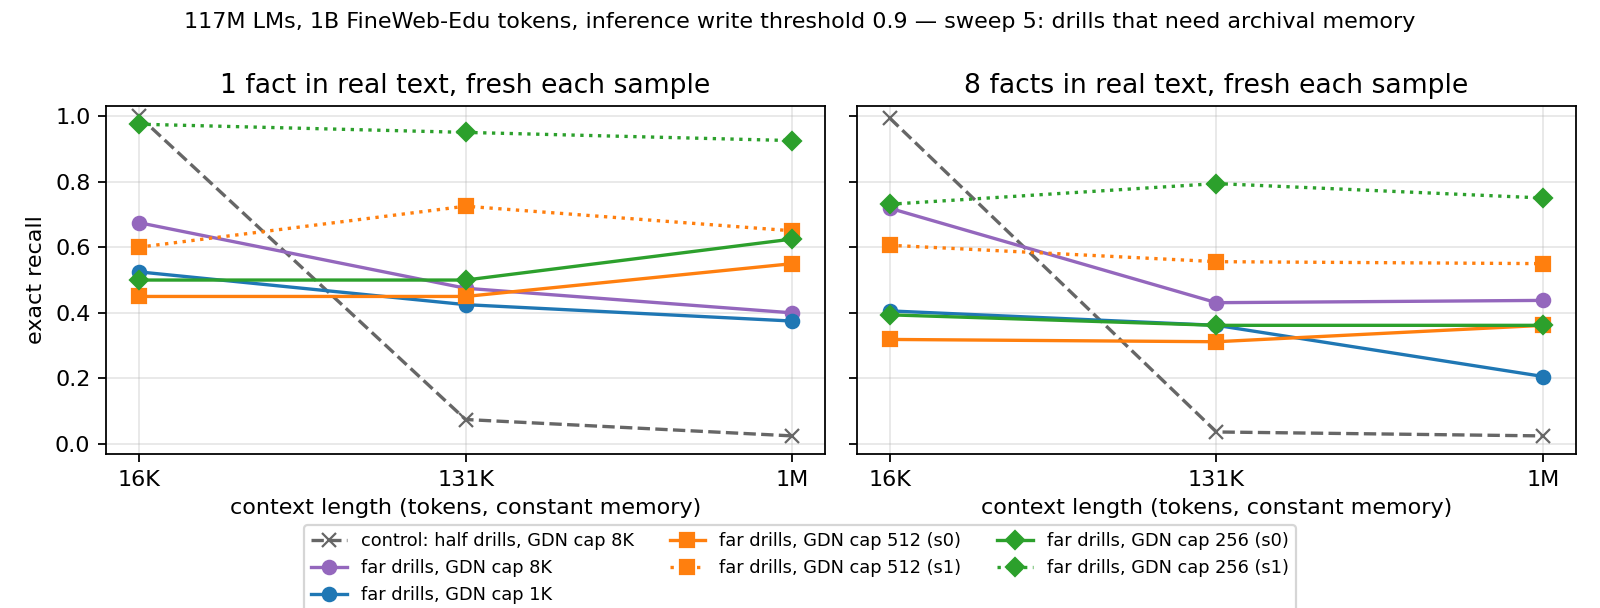
\includegraphics[width=\linewidth]{fig_sweep5_far_drills.png}
\caption{117M language models (1B FineWeb-Edu tokens). With far drills and a GDN cap of 256 or 512 tokens, recall is flat from 16K to 1M tokens; with caps of 1K and 8K it falls with distance; the standard-drill control collapses beyond 16K. The level varies across runs.}
\label{fig:routing}
\end{figure}

With a GDN cap of 256 or 512 tokens, all six far-drill runs are flat from 16K to 1M: the four in \cref{tab:routing} and two further seeds at cap 512, which score 0.325 / 0.275 / 0.275 and 0.725 / 0.70 / 0.875 at 16K / 131K / 1M ($K = 1$). None of the six has 1M recall significantly below its 16K recall (one-sided Fisher exact test on $K = 1$, all $p \ge 0.3$). With caps of 8K and 1{,}024 tokens, recall falls with distance (cap 8K: 27/40 at 16K versus 16/40 at 1M, $p = 0.012$). The recall \emph{level} still varies across runs (0.275--0.925 at 1M for the six); the distance profile does not. Wholly unseen sentence templates stay near 0 ($\le 0.013$ in the two far-drill runs evaluated on them).

\paragraph{What the working models do.} Over four 1M-token streams, a working model stores each fact in about 10 heads and writes on 1.2\% of text tokens; an older recipe stores it in about 30 heads and writes on 7.1\% of text tokens. With retention simulated at write threshold 0.9, only about one head of the working model keeps retention above 0.9 at 1M (about 11 for the older recipe), yet its recall is 0.98 ($n = 40$), against about 0.35 ($n = 20$) for the older recipe. Retention is not the bottleneck: one surviving head suffices once the read is clean.

\subsection{Scale}
At 494M parameters (6B tokens), the routing fix carries over (\cref{tab:scale}). Recall is flat from 16K to 1M tokens, whereas the earlier 494M runs failed beyond 16K. We did not train a matched 494M GDN baseline; at 117M the matched GDN is already near zero at 16K (\cref{tab:levers}).

\begin{table}[t]
\centering
\caption{494M models: recall $K = 1$ / $K = 8$ at inference threshold 0.9, and validation perplexity.}
\label{tab:scale}
\resizebox{\linewidth}{!}{\begin{tabular}{@{}lcccc@{}}
\toprule
Model & 16K & 131K & 1M & Val.\ ppl \\
\midrule
standard drills, 40 phrasings, cap 8K (v1, 10B tokens) & 0.53 / 0.38 & 0.08 / 0.08 & 0.05 / 0.07 & 24.2 \\
\textbf{far drills + GDN cap 256 (v4)} & 0.85 / 0.79 & 0.88 / 0.74 & \textbf{0.88 / 0.74} & 27.0 \\
\bottomrule
\end{tabular}}
\end{table}

\subsection{Unseen phrasings}
From-scratch models do not generalise to fact phrasings unseen in training. With 10 templates, recall on 3 unseen sentence frames is about 0 ($\le 0.025$); with 318 compositional phrasings, recall on unseen frames $\times$ unseen attributes is at most 0.18 at 16K and at most 0.10 beyond (10 runs). The write gate learns \emph{which phrasings to store}, not \emph{what a fact is}. Pretrained features change this (\cref{sec:graft}).

\section{Grafting the memory onto frozen pretrained models}
\label{sec:graft}
\subsection{\KH{} on Liquid LFM2}
We graft archival adapters onto LFM2-350M (1{,}024-token chunks, 16 heads per adapter, 16M trainable parameters) and LFM2-1.2B (2{,}048-token chunks, 32 heads, 63M trainable parameters) \citep{lfm2}. \Cref{tab:kh1} reports recall; \cref{fig:kh1} plots it against distance.

\begin{table}[t]
\centering
\small
\caption{\KH{} recall, $K = 1$ / $K = 8$ (40 / 20 streams), facts spliced into FineWeb-Edu. ``Train $\to$ inference'' gives the last training threshold and the inference threshold. ``Chat'' renders the question as a chat turn; other rows are plain questions. The memory-off row is LFM2-350M. All rows use the development evaluation streams and the seed-0 models; \cref{tab:seeds} gives fresh-stream and multi-seed results.}
\label{tab:kh1}
\begin{tabular}{@{}llccc@{}}
\toprule
Model (train $\to$ inference $\tauw$) & Phrasings & 16K & 131K & 1M \\
\midrule
350M, 0.9 $\to$ 0.97 & trained & -- & 1.00 / 0.80 & 0.75 / 0.70 \\
350M, 0.9 $\to$ 0.97 & trained, chat & 0.90 / 0.90 & 0.975 / 0.78 & 0.875 / 0.74 \\
\textbf{350M, 0.97 $\to$ 0.99} & trained & 0.95 / 0.84 & 1.00 / 0.91 & \textbf{0.925 / 0.77} \\
\textbf{350M, 0.97 $\to$ 0.99} & trained, chat & 0.975 / 0.91 & 0.975 / 0.81 & \textbf{0.95 / 0.78} \\
350M, 0.9 $\to$ 0.97 & unseen & 0.65 / 0.44 & 0.55 / 0.36 & 0.30 / 0.30 \\
\textbf{350M, 0.97 $\to$ 0.99} & unseen & 0.80 / 0.45 & 0.80 / 0.41 & \textbf{0.575 / 0.325} \\
\midrule
1.2B, 0.9 $\to$ 0.97 & trained, chat & 0.95 / 0.94 & 0.975 / 0.86 & 0.575 / 0.51 \\
1.2B, 0.9 $\to$ 0.97 & unseen & 0.725 / 0.55 & 0.70 / 0.44 & 0.175 / 0.18 \\
\textbf{1.2B, 0.97 $\to$ 0.99} & trained, chat & 0.95 / 0.91 & 0.95 / 0.86 & \textbf{0.85 / 0.71} \\
\textbf{1.2B, 0.97 $\to$ 0.99} & unseen & 0.875 / 0.59 & 0.825 / 0.475 & \textbf{0.45 / 0.39} \\
\midrule
memory off (plain chunked LFM2) & trained & 0.00 / 0.00 & -- & -- \\
\bottomrule
\end{tabular}
\end{table}

\begin{figure}[t]
\centering
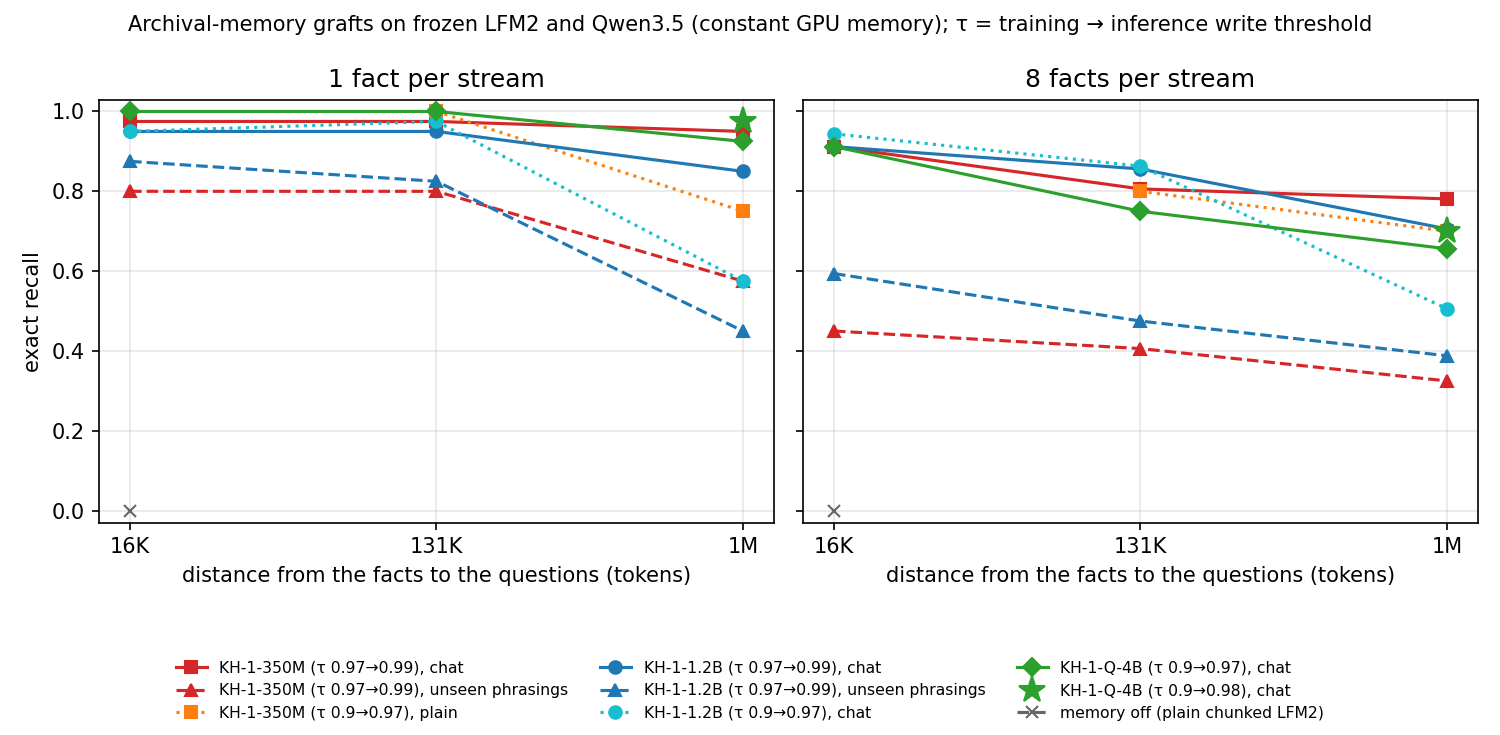
\includegraphics[width=\linewidth]{fig_kh1_recall.png}
\caption{Recall of the grafts versus distance on the development streams ($n = 40$ per point; fresh-stream and multi-seed results are in \cref{tab:seeds}). With the write-threshold curriculum (trained at $\tauw = 0.97$, run at 0.99), the LFM2 grafts (red: 350M; blue: 1.2B) stay high to 1M tokens, while the same models one stage earlier (trained at 0.9, run at 0.97; dotted) fade at 1M. The Qwen3.5-4B graft (green) reaches 0.975 at 1M when run at 0.98 (star; 0.90 on fresh streams). Dashed: unseen phrasings. Grey: memory switched off (measured at 16K).}
\label{fig:kh1}
\end{figure}

\paragraph{Pretrained features partly solve phrasing generalisation.} Unseen frames $\times$ attributes reach 0.55--0.875 at 16K across models and seeds, and 0.375--0.575 at 1M with the threshold curriculum, where from-scratch models reach at most 0.18 at 16K and at most 0.10 beyond. Wholly unseen sentence templates reach 0.43--0.55 at 16K for most LFM2 grafts but at most 0.05 at 1M.

\paragraph{Inside novels.} On a harder haystack, 1M-token windows of three Project Gutenberg novels \citep{gutenberg} that are dense with proper names, recall is lower than on FineWeb-Edu ($K = 1$, chat questions, $n = 40$). The 350M graft scores 0.775 (trained at 0.9, run at 0.97) and 0.825 (trained at 0.97, run at 0.99); the 1.2B graft scores 0.90 (trained at 0.97, run at 0.99).

\subsection{Why one threshold step fades: the write gate learns a shortcut}
\label{sec:shortcut}
With a single threshold step (train at 0.9, run at 0.97), recall is 0.95--1.00 at 131K but 0.50--0.75 at 1M, while the best from-scratch models stay flat. Write statistics (\texttt{write\_stats.py}, three 1M-token streams; \texttt{probe\_text\_writes.py}, 131K tokens) explain why.
\begin{itemize}
\item Training facts use made-up names and mostly numeric values, so the gate fires on rare proper nouns and numbers in ordinary text: 6.6--6.9\% of tokens trigger at least one archival head, in FineWeb-Edu as in \emph{War and Peace}, where most writes land on fragments of Russian names.
\item The surviving text writes are saturated ($\beta$ between 0.97 and 0.99), about 0.13\% of tokens per head: some 1{,}300 writes per head per 1M tokens against 64-dimensional keys.
\item After 1M tokens, the median written head keeps only 2--7\% of the fact's key direction, and only about 1\% of written heads keep more than 0.9. From-scratch models keep the fact in 12.5\% of written heads.
\end{itemize}

\subsection{Train one threshold step below the inference threshold}
\label{sec:curriculum}
For the seed-0 model, fine-tuning the 350M graft at $\tauw = 0.97$ for 100M tokens and running it at 0.99 makes $K = 1$ recall nearly flat from 16K to 1M (0.95 / 1.00 / 0.925; 0.975 / 0.975 / 0.95 with chat questions). At 1M it raises recall from 0.75 to 0.925 with plain questions and from 0.875 to 0.95 with chat questions, and nearly doubles recall on unseen phrasings (0.30 $\to$ 0.575). The same step (300M tokens) lifts the 1.2B graft from 0.575 to 0.85 at 1M (chat questions) and from 0.175 to 0.45 on unseen phrasings. Running the 1.2B graft at 0.995 instead raises 1M recall further (plain questions: 0.90 versus 0.80) at the cost of short-range recall (0.525 at 16K), so we keep 0.99.

The gain is in the readout, not in retention. At 1M tokens the median written head keeps about 0.08 of the fact's key when the model runs at 0.99, against about 0.07 before the step (run at 0.97). Training at 0.97 admits about 13 times more text writes than inference at 0.99 (2.3\% versus 0.18\% of tokens per head), so the readout learns to recover facts from a much noisier state than it meets at test time. At its own training threshold the same model fails at 1M (0.175).

What does not help: a second step (train at 0.99, run at 0.995); a stronger L1 penalty on text writes (0.6 instead of 0.2); a logit-space BCE penalty on text writes; and training facts about real-looking names. The BCE penalty lowers fact writes along with text writes (median fact write strength 0.984 versus 0.992); we expect the same of the stronger L1 penalty but did not measure it. Mixing thresholds across heads at inference (half the heads at 0.995) breaks the readout, which is tuned to the state statistics of a uniform threshold: on the book demo of \cref{sec:demo} it drops the 350M graft from 3 of 5 to 0 of 5.

\paragraph{Seeds and fresh streams.} We retrained the full 350M recipe (all four stages) with two further seeds, and re-measured the three released models on 40 fresh streams (a different sampler seed), since their inference thresholds had been chosen on the development streams (\cref{tab:seeds}). The threshold step raises 1M recall in every seed (chat questions: $+0.075$, $+0.125$, $+0.175$), and short-range recall is stable (0.95--0.975 at 16K), but the 1M level varies across seeds from 0.575 to 0.95. On fresh streams the one-fact numbers drop by 0.05--0.10 and the eight-fact numbers by at most 0.03. The released 350M model is the best of the three seeds. These differences sit close to the noise floor: with 40 streams, a one-fact recall near 0.7 has a 95\% binomial interval of about $\pm 0.14$, and retraining only the last stage of seed 2 with the same seed moved its 1M recall from 0.575 to 0.75. Single-run one-fact differences below about 0.15 should therefore be read as noise; eight-fact cells (160 facts) are tighter, and consistent signs across seeds carry more weight than any single gap.

\begin{table}[t]
\centering
\small
\caption{Robustness of the graft results. Top: the 350M recipe trained with three seeds (trained at 0.97, run at 0.99; recall $K = 1$, 40 streams; $K = 8$ in parentheses). Bottom: the released models at 1M tokens on the development streams and on 40 fresh streams ($K = 1$ / $K = 8$, chat questions).}
\label{tab:seeds}
\begin{tabular}{@{}lcccc@{}}
\toprule
350M recipe & seed 0 & seed 1 & seed 2 & mean $\pm$ s.d. \\
\midrule
chat, 16K & 0.975 & 0.975 & 0.95 & 0.967 $\pm$ 0.014 \\
chat, 131K & 0.975 & 0.90 & 0.925 & 0.933 $\pm$ 0.038 \\
chat, 1M & 0.95 (0.78) & 0.675 (0.64) & 0.575 (0.58) & 0.733 $\pm$ 0.194 \\
chat, 1M, one stage earlier (0.9 $\to$ 0.97) & 0.875 & 0.55 & 0.40 & 0.608 $\pm$ 0.243 \\
plain, 1M & 0.925 & 0.825 & 0.70 & 0.817 $\pm$ 0.113 \\
unseen phrasings, 1M & 0.575 & 0.375 & 0.45 & 0.467 $\pm$ 0.101 \\
inside novels, 1M & 0.825 & 0.65 & 0.80 & 0.758 $\pm$ 0.095 \\
\midrule
Released model, 1M & \multicolumn{2}{c}{development streams} & \multicolumn{2}{c}{fresh streams} \\
\midrule
350M (0.97 $\to$ 0.99) & \multicolumn{2}{c}{0.95 / 0.78} & \multicolumn{2}{c}{0.90 / 0.75} \\
1.2B (0.97 $\to$ 0.99) & \multicolumn{2}{c}{0.85 / 0.71} & \multicolumn{2}{c}{0.75 / 0.70} \\
Qwen3.5-4B (0.9 $\to$ 0.98) & \multicolumn{2}{c}{0.975 / 0.70} & \multicolumn{2}{c}{0.90 / 0.70} \\
\bottomrule
\end{tabular}
\end{table}

\paragraph{What differs between seeds.} Per-head write statistics (\texttt{write\_stats.py}, the same six 1M-token streams for every model, one planted fact each) show a robust relation \emph{within} a model: a fact-storing head's text-write rate correlates negatively with its retention of the fact at 1M ($r = -0.41$ to $-0.51$ over heads, in each of the three seeds), as the erasure term of the delta rule predicts, and the heads that keep a fact write about 13 text tokens per million. Across models the picture is weaker (\cref{tab:quiet}). The two seed-0 models have the highest median retention at 1M (0.063 and 0.049, against 0.006--0.034 for the other eight) and the highest recall, but over all ten 350M models (three seeds, two reruns of stage 4 and the variants below), 1M recall does not track the number of \emph{quiet fact heads}, heads that store the fact in at least half of the streams and write under 0.01\% of text tokens (Spearman $\rho = 0.02$ for one fact, 0.11 for eight), and tracks median retention only weakly ($\rho = 0.33$ and 0.39; $n = 10$, not significant). A ranking we first saw on the three seeds alone did not survive the larger set. What makes seed 0 better remains open.

\begin{table}[t]
\centering
\small
\caption{The ten 350M-recipe models: 1M recall (chat; mean of development and fresh streams where both were measured) and write statistics over the same six 1M-token streams (48 archival heads, inference at 0.99; two-tier at 0.99 / 0.998). Quiet fact heads: store the fact in $\ge$ 50\% of streams and write $<$ 0.01\% of text tokens.}
\label{tab:quiet}
\begin{tabular}{@{}lcccc@{}}
\toprule
Model (stage 4) & 1M, $K = 1$ & 1M, $K = 8$ & quiet fact heads & median retention at 1M \\
\midrule
seed 0 & 0.93 & 0.77 & 10 & 0.063 \\
seed 0, two-tier & 0.95 & 0.80 & 6 & 0.049 \\
seed 1 & 0.68 & 0.64 & 6 & 0.006 \\
seed 1, rerun & 0.73 & 0.57 & 5 & 0.015 \\
seed 1, two-tier & 0.71 & 0.66 & 9 & 0.027 \\
seed 1, quiet-head penalty & 0.54 & 0.50 & 8 & 0.034 \\
seed 2 & 0.58 & 0.58 & 4 & 0.014 \\
seed 2, rerun & 0.68 & 0.56 & 6 & 0.015 \\
seed 2, two-tier & 0.73 & 0.62 & 4 & 0.011 \\
seed 2, quiet-head penalty & 0.71 & 0.68 & 2 & 0.019 \\
\bottomrule
\end{tabular}
\end{table}

\paragraph{Making fact heads quieter by design.} Following the within-model relation, we tried two ways to make fact heads write less ordinary text, each by redoing only stage 4 of seeds 1 and 2 and comparing against a rerun of the standard stage 4 (same seed and data): two-tier thresholds (half of each layer's heads train at 0.995 and run at 0.998, the rest at 0.97 and 0.99), and a five-fold text-write penalty on half of each layer's heads. Two-tier thresholds beat the rerun control on eight-fact recall at 1M in all four comparisons (two seeds, development and fresh streams; $+0.06$ to $+0.09$) and give the best 350M result on seed 0 (0.975, 0.925 on fresh streams), but their one-fact gains are within noise. On LFM2.5-8B-A1B (\cref{sec:lfm25}) one two-tier run raised 1M recall from 0.375 to 0.675 (0.525 on fresh streams), but a second seed gave 0.275 while a rerun of the standard stage gave 0.35, so the gain did not replicate. The extra penalty is mixed and lowers short-range recall. Write statistics show why both are partial: the strict tier writes 4--7 times less ordinary text but also stores facts less often, and the penalty raises retention but lowers the number of heads that store each fact. Both trade fact writes for quiet, because the write gate cannot yet tell a fact from a rare name or number (\cref{sec:shortcut}); separating them is the open problem for the next version.

\subsection{An end-to-end check on a consumer GPU}
\label{sec:demo}
We greet the model in chat, then stream 1{,}318{,}920 tokens (\emph{War and Peace}, \emph{Moby Dick} and \emph{Pride and Prejudice}) with five facts planted at token 16{,}814, and finally ask the five questions as chat turns, about 1.30M tokens after the facts. Four facts use trained phrasings and one uses a phrasing never seen in training. On an 8\,GB RTX 3070 Ti, the 1.2B graft (trained at 0.97, run at 0.99) answers 4 of 5 exactly, including the made-up three-token password \emph{thuzoka}; it misses the unseen phrasing (``2879'' for 287). It reads the stream in 96\,s (13.7K tokens/s) at a constant 2.60\,GB (peak 2.81\,GB). The 350M graft answers 3 of 5 in 0.84\,GB at 32.5K tokens/s. With the memory switched off (ReZero gates zeroed, which leaves plain chunked LFM2), both models answer 0 of 5 and invent answers (the 1.2B model: ``12'', ``KRIBRISEN-WIFI'', ``123.456 MHz''). A five-fact demonstration is anecdotal; \cref{tab:kh1} gives the statistics. Because every chat turn is also written to memory, the order of the questions can change later answers.

\paragraph{Controls and language-modelling quality.} With the memory switched off, recall at 16K is 0.00 (LFM2-350M). The adapters cost no language-modelling quality: measured over the second 1M tokens of a 2M-token stream, they lower validation perplexity by 5--9\% relative to zeroing them (\cref{tab:ppl}). Part of that comes from the adapters' processing within a chunk. To isolate the memory, we keep the adapters on but clear the memory before every chunk: carrying it across chunks accounts for 2--5\% (for example 14.34 $\to$ 13.64 for the 1.2B graft trained at 0.9), about half of the total for the LFM2 grafts. The memory recovers part of the cross-chunk context that chunking removes.

\begin{table}[t]
\centering
\small
\caption{Validation perplexity (FineWeb-Edu, second 1M tokens of a 2M-token stream). ``Cleared'': adapters on, memory state cleared before every chunk, so the difference to ``carried'' is the cross-chunk memory alone.}
\label{tab:ppl}
\begin{tabular}{@{}lccc@{}}
\toprule
Graft & memory carried & memory cleared & adapters off \\
\midrule
350M, trained at 0.9 & 20.52 & 21.60 & 22.64 \\
1.2B, trained at 0.9 & 13.64 & 14.34 & 15.00 \\
1.2B, released (trained at 0.97) & 13.66 & 14.22 & 15.00 \\
Qwen3.5-4B, stage 3 & 9.81 & 10.00 & 10.29 \\
\bottomrule
\end{tabular}
\end{table}

\subsection{\KH{}-Q on Qwen3.5-4B}
\label{sec:qwen}
Qwen3.5-4B \citep{qwen35} interleaves 24 Gated DeltaNet layers with 8 full-attention layers. We run it frozen on 2{,}048-token chunks with every GDN state reset and no key--value cache across chunks, and add three 40-head archival adapters (99M trainable parameters). Training runs at about 290K tokens/s on eight B200 GPUs: stage 1 ($\tauw = 0.5$, 1.5B tokens, 86 min) and stage 2 ($\tauw = 0.9$, 0.5B tokens, 28 min).

\begin{table}[t]
\centering
\small
\caption{\KH{}-Q (Qwen3.5-4B) recall, $K = 1$ / $K = 8$ (40 / 20 streams), FineWeb-Edu.}
\label{tab:qwen}
\resizebox{\linewidth}{!}{\begin{tabular}{@{}llccc@{}}
\toprule
Stage (train $\to$ inference $\tauw$) & Questions & 16K & 131K & 1M \\
\midrule
s1 (0.5 $\to$ 0.9) & plain & 0.95 / 0.70 & 0.975 / 0.79 & 0.925 / 0.69 \\
s2 (0.9 $\to$ 0.97) & chat & 1.00 / 0.91 & 1.00 / 0.75 & 0.925 / 0.66 \\
\textbf{s2 (0.9 $\to$ 0.98)} & chat & -- & -- & \textbf{0.975 / 0.70} \\
s2 (0.9 $\to$ 0.97) & unseen frames $\times$ attributes & 0.80 / 0.57 & 0.875 / 0.47 & 0.575 / 0.45 \\
s3 (0.97 $\to$ 0.99) & wholly unseen sentence templates & 0.675 / 0.28 & 0.50 / 0.22 & 0.10 / 0.10 \\
memory off & plain & 0.00 / 0.01 & 0.00 / 0.03 & 0.00 / 0.01 \\
\bottomrule
\end{tabular}}
\end{table}

A stronger base gives long-range recall early: stage 1 alone reaches 0.925 at 1M, where LFM2-1.2B reached 0.425 at the same stage. On wholly unseen sentence templates the 4B graft reaches 0.675 at 16K and 0.50 at 131K, but only 0.10 at 1M (the LFM2 grafts: 0.43--0.55 at 16K, at most 0.40 at 131K and 0.05 at 1M). The threshold step of \cref{sec:curriculum} does not transfer as is: a third stage trained at 0.97 collapses 1M recall to 0.25--0.45 at inference thresholds 0.99--0.995, while the stage-2 model peaks at inference threshold 0.98 among 0.97, 0.98 and 0.99 (0.975 at 1M; 3 of 5 on the book demo). Because this threshold was chosen on the evaluation streams, we re-measured it on 40 fresh streams: 0.90 / 0.70 (\cref{tab:seeds}). The inference threshold is a per-model setting that is cheap to sweep. The adapters lower validation perplexity of the stage-3 model from 10.29 to 9.81, of which the cross-chunk memory accounts for 10.00 $\to$ 9.81 (\cref{tab:ppl}). With the frozen base quantised to 4-bit NF4 \citep{qlora2023}, the graft runs on the 8\,GB RTX 3070 Ti at 3.9\,GB peak and about 4.1K tokens/s, and answers 2 of 5 on the book demo at threshold 0.98 (3 of 5 in bf16).

\subsection{A mixture-of-experts base: LFM2.5-8B-A1B}
\label{sec:lfm25}
LFM2.5-8B-A1B is a sparse mixture-of-experts model (8.5B parameters, about 1B active per token; 24 layers, of which 6 use attention; 128K-token vocabulary). We add three 32-head archival adapters after layers 11, 17 and 23 (63M trainable parameters) and run it on 2{,}048-token chunks. On one H200 (48K tokens/s) we trained 450M tokens at $\tauw = 0.5$, 200M at 0.9 and 100M at 0.97: 750M tokens in total with 32K-token batches, against 2B tokens and 131K-token batches for the Qwen3.5-4B graft.

\begin{table}[t]
\centering
\small
\caption{\KH{} on LFM2.5-8B-A1B (mixture of experts), recall $K = 1$ / $K = 8$ (40 / 20 streams), chat questions unless noted.}
\label{tab:lfm25}
\begin{tabular}{@{}lccc@{}}
\toprule
Stage (train $\to$ inference $\tauw$) & 16K & 131K & 1M \\
\midrule
s2 (0.9 $\to$ 0.98) & 0.425 / 0.55 & 0.375 / 0.325 & 0.275 / 0.33 \\
s3 (0.97 $\to$ 0.99) & 0.675 / 0.875 & 0.55 / 0.57 & 0.375 / 0.36 \\
s3, fresh streams & -- & -- & 0.375 / 0.33 \\
s3, plain questions & -- & -- & 0.325 / 0.25 \\
s3, unseen frames $\times$ attributes & 0.175 / 0.27 & -- & 0.20 / 0.18 \\
memory off & 0.00 / 0.006 & -- & -- \\
\bottomrule
\end{tabular}
\end{table}

The memory transfers to the mixture-of-experts base (0.675 at 16K and 0.375 at 1M, against 0.00 without it; \cref{tab:lfm25}), and the threshold step helps again (1M: 0.275 $\to$ 0.375), but long-range recall stays far below the dense grafts. Training accuracy by fact age shows where: facts asked in the next chunk are answered (1.00), facts 16K--127K tokens back only 0.58 of the time. Its write statistics point the same way: fact-storing heads write 0.97\% of text tokens (the 350M models of \cref{tab:quiet}: 0.19--0.57\%), only 2 of the 96 heads are quiet fact heads, and median retention at 1M is 0.0017 (350M models: 0.006--0.063). With this short training run, the write gate has not learned to keep ordinary text out of the fact heads. The LFM2.5 bases are also poorly calibrated on plain text (LFM2.5-8B-A1B: loss 3.73 on \emph{Pride and Prejudice} with a BOS per chunk; LFM2.5-350M: 6.29 on a 4{,}096-token window of the same book, against 3.40 for LFM2-350M, although it chats normally), so on this base the adapters' language-modelling loss mostly recalibrates the output: perplexity falls from 42.5 (adapters off) to 17.7 (memory cleared every chunk) and 12.7 (memory carried). A rerun of stage 3 reproduces the 1M result (0.35 / 0.39). We read the gap to the dense grafts as a training-budget gap rather than a property of the architecture: the Qwen3.5-4B graft, also a hybrid base, reached 0.90 on fresh streams with 2B tokens and 131K-token batches on eight B200s, against 750M tokens and 32K-token batches here; we have not tested a matched budget. We do not use LFM2.5-350M as a base for this reason.

\subsection{An attention-only base: Gemma 4 E2B}
\label{sec:gemma}
Gemma 4 E2B \citep{gemma4} is an attention-only model (35 layers, sliding-window attention with a global layer every fifth layer, per-layer embeddings, key--value sharing across its last layers, 262K-token vocabulary). Because of that machinery we do not re-implement its layer loop: the adapters run as forward hooks inside Gemma's own forward pass on [BOS] + chunk, with no key--value cache across chunks (with the gates at zero the graft reproduces the native chunked loss exactly). We add three 24-head adapters after layers 16, 25 and 34 (36M trainable parameters) and train on one H200 (25K tokens/s): 600M tokens at $\tauw = 0.5$, 250M at 0.9 and 150M at 0.97, with 16K-token batches.

\begin{table}[t]
\centering
\small
\caption{\KH{} on Gemma 4 E2B, recall $K = 1$ / $K = 8$ (40 / 20 streams), chat questions unless noted.}
\label{tab:gemma}
\begin{tabular}{@{}lccc@{}}
\toprule
Stage (train $\to$ inference $\tauw$) & 16K & 131K & 1M \\
\midrule
s1 (0.5 $\to$ 0.9) & 0.00 / 0.04 & -- & -- \\
s3 (0.97 $\to$ 0.99) & 0.575 / 0.49 & 0.55 / 0.40 & 0.575 / 0.42 \\
s3, fresh streams & -- & -- & 0.40 / 0.44 \\
s3, unseen frames $\times$ attributes & 0.20 / 0.24 & -- & 0.225 / 0.20 \\
memory off & 0.00 / 0.006 & -- & -- \\
\bottomrule
\end{tabular}
\end{table}

Stage 1 alone stores almost nothing (0.00 at 16K); the threshold curriculum switches the memory on, and after stage 3 recall is flat from 16K to 1M (\cref{tab:gemma}), at a level between the LFM2.5-8B graft and the dense LFM2 and Qwen3.5 grafts. As for LFM2.5, the run had about half of the Qwen3.5 graft's tokens and an eighth of its batch size.

\section{A standard benchmark: BABILong}
\label{sec:babilong}
BABILong \citep{babilong2024} hides bAbI stories (``Mary went to the bathroom.'') in PG19 books and asks a one-word question at the end; qa1--qa5 need one to three supporting facts. We stream each test sample through the 350M graft and ask its question as a chat turn, so the frozen base never sees the story and the question together unless the whole sample fits in one chunk; an answer counts if the target is among its first words. Baselines on the same samples: the base with the memory off, and retrieval (BM25, ten best sentences in story order, put in the prompt of the same base).

\begin{table}[t]
\centering
\small
\caption{BABILong test split, mean accuracy over qa1--qa5 (50 samples per task and length; 20 at 1M). Fine-tuning trains only the 16M adapter parameters on the BABILong training split; inference threshold 0.97.}
\label{tab:babilong}
\begin{tabular}{@{}lcccccc@{}}
\toprule
 & 0K & 4K & 16K & 64K & 128K & 1M \\
\midrule
\KH{}-350M, no BABILong training & 0.03 & 0.00 & 0.00 & -- & -- & -- \\
memory off & 0.02 & 0.02 & 0.02 & -- & -- & -- \\
RAG (BM25 top-10, same base) & 0.36 & 0.24 & 0.23 & 0.20 & 0.21 & 0.25 \\
fine-tuned, 6K samples (0K--16K) & 0.41 & 0.43 & 0.40 & 0.34 & 0.32 & -- \\
+ 12K samples (0K--32K) & 0.55 & 0.54 & 0.48 & 0.47 & 0.42 & 0.26 \\
\textbf{+ 4K samples (16K--64K)} & \textbf{0.60} & \textbf{0.55} & \textbf{0.58} & \textbf{0.61} & \textbf{0.57} & \textbf{0.50} \\
\bottomrule
\end{tabular}
\end{table}

Out of the box \KH{} answers nothing (\cref{tab:babilong}): its gate learned to store ``a name's attribute is a value'', not story sentences. Fine-tuning only the adapters on the training split (22K samples in three rounds, about four hours on one shared H200) makes recall flat from 0K to 1M at 0.50--0.61, between two and three times the retrieval baseline at every length from 4K; training on longer samples removed the fade with length. By task, qa5 reaches 0.96--0.98 to 128K (0.95 at 1M) and qa4 0.64--0.84, while qa1 stays near 0.5 (0.45 at 1M) and the multi-hop qa2 and qa3 at 0.25--0.45. Recurrent-memory Transformers fine-tuned on BABILong reach about 0.9 on qa1 at 1M \citep{babilong2024,armt2024}; our numbers come from a 350M frozen base with a 1.9\,MB memory and a short fine-tune.

\section{Related work}
\label{sec:related}
\paragraph{Recall in efficient sequence models.} Associative-recall benchmarks such as MQAR \citep{zoology2023} and the recall--throughput analysis of \citet{based2024} show that fixed-state models trade recall for memory; \citet{jelassi2024} prove and measure a copying gap to Transformers, large-scale comparisons find the same weakness in Mamba-based language models \citep{waleffe2024}, and \citet{jrt2024} narrow the gap by letting a recurrent model read its context twice. We target a different regime: a few facts read once, recalled after very long, arbitrary text, where the limiting factor is how the state is written rather than its size.

\paragraph{Fixed-state and delta-rule models.} Our memory builds on fast-weight programmers and the delta rule \citep{widrowhoff1960,schmidhuber1992,schlag2021}, its parallel and gated forms \citep{deltanet2024,gdn2024,gla2023}, and selective state spaces \citep{mamba2023,mamba2_2024,mamba3_2025}; RWKV-7 \citep{rwkv7_2025} also uses a generalised delta rule, and hybrid models such as Jamba and Samba \citep{jamba2024,samba2024} interleave state-space and attention layers, as Qwen3.5 interleaves Gated DeltaNet and attention. Titans and ATLAS \citep{titans2024,atlas2025} learn a neural memory at test time, MesaNet \citep{mesanet2025} solves an in-context regression objective optimally, and log-linear attention \citep{loglinear2025} lets the state grow logarithmically. StateX \citep{statex2025} expands the recurrent state after training to improve recall. Our archival heads keep a fixed state and change only what may be written and what decays.

\paragraph{Length extrapolation of recurrent models.} DeciMamba \citep{decimamba2024} and LongMamba \citep{longmamba2025} extend Mamba's receptive field without training; \citet{stuffedmamba2024} trace the failure of recurrent models beyond their training length to states too large to learn to forget within it; \citet{buitrago2025} show that recurrent models fail to extrapolate when they have not seen the states reached at long lengths, and improve extrapolation with interventions such as state passing. Our routing principle concerns the training signal of \emph{writes} rather than the state distribution, and our traps (\cref{sec:traps}) are failure modes of the long-range training curriculum itself.

\paragraph{Memory-augmented Transformers.} Memorizing Transformers \citep{memorizingtf2022} retrieve from an external key--value store, Infini-attention \citep{infiniattention2024} adds a compressive memory to each attention layer, the Recurrent Memory Transformer \citep{rmt2022} and ARMT \citep{armt2024} pass memory tokens or associative memory across segments, and hardware-aligned hierarchical sparse attention gives recurrent models efficient access to long-term memory \citep{hsa_ramba2025}. Closest to our grafts, LongMem \citep{longmem2023} augments a frozen language model with a decoupled long-term memory read by a trainable side network, and recurrent memory on a pretrained Transformer retrieves facts from up to 2M tokens \citep{rmtscaling2024}. Our grafts differ in mechanism: a fixed-size associative state written by a thresholded delta rule and trained by the routing principle, inserted as adapters \citep{adapters2019,lora2021} into a frozen model that runs chunk-locally, with no retrieval store and no memory tokens.

\paragraph{Interference and orthogonal subspaces.} Keeping stored items safe from later writes resembles orthogonal-subspace methods for continual learning such as OWM and GPM \citep{owm2019,gpm2021}; our write threshold and text-write penalty act on the same erasure term, but per token at inference time.

\paragraph{Long-context evaluation.} Needle-in-a-haystack tests \citep{niah2023}, RULER \citep{ruler2024} and BABILong \citep{babilong2024} evaluate retrieval and reasoning over long contexts. Most of our facts are synthetic templates spliced into real text; \cref{sec:babilong} adds BABILong.

\section{Limitations}
\label{sec:limitations}
\begin{itemize}
\item \textbf{Facts, not documents.} The memory recalls stored name--attribute--value facts. It does not let the model re-read or summarise a long document.
\item \textbf{Phrasings.} Recall is strongest for trained phrasings. Unseen combinations reach 0.375--0.575 at 1M with pretrained bases, and wholly unseen sentence templates are near zero at 1M.
\item \textbf{Level versus profile.} With the full recipe, recall \emph{profiles} are flat across distance, but recall \emph{levels} vary across runs and models (0.275--0.925 at 1M for the six from-scratch far-drill runs with a short GDN cap).
\item \textbf{Capacity and competition.} This is a fixed-state memory: distance-invariant, not unbounded in content. Name-dense text competes for it (0.825 inside novels versus 0.95 on FineWeb-Edu for the 350M graft), and every chat turn is written to it as well.
\item \textbf{Evaluation.} Most results use synthetic facts spliced into real text. On BABILong (\cref{sec:babilong}) the memory needs fine-tuning on the task's own sentences and reaches 0.50--0.61; RULER-style evaluation is future work. Decoy robustness at 1M is unsolved.
\item \textbf{Seeds.} The 350M recipe's 1M recall varies across training seeds (0.575--0.95 with chat questions), retraining only its last stage moves it by up to 0.175, and per-head write statistics do not explain the spread across models (\cref{tab:quiet}); the released model is the best of three. The 1.2B and Qwen3.5-4B grafts were trained once.
\end{itemize}

\section{Conclusion}
A fixed-state memory can recall facts after a million tokens of arbitrary text when two conditions hold: the heads that hold facts neither decay nor accept routine writes, and training makes those heads, rather than any bounded-memory layer, the way to answer. The same principle turns frozen pretrained models into constant-memory fact readers with small adapters that run on a consumer GPU. On BABILong a short adapter fine-tune gives recall that is flat to 1M at two to three times a retrieval baseline. Recall of phrasings unseen in training, decoys, and multi-hop questions remain open.

\section*{Code, data and models}
Code, training logs, evaluation outputs and the research log: \url{https://github.com/01TEK/KH} (tag \texttt{v2.3}).\\
Adapters: \url{https://huggingface.co/01TEK} (\texttt{KH-1-350M}, \texttt{KH-1-1.2B}, \texttt{KH-1-Q-4B}).\\
Live demo: \url{https://huggingface.co/spaces/01TEK/KH-1-live}.\\
Demo video: \url{https://youtu.be/mCGc3_Mh0HI}.\\
This preprint: \href{https://doi.org/10.5281/zenodo.23447665}{doi:10.5281/zenodo.23447665}.

\section*{Acknowledgements}
We thank Nebius for the GPU credits, provided through the NVIDIA Inception program, that paid for the NVIDIA H200 and B200 compute used in this work; the remaining experiments ran on a local RTX 3070 Ti. Much of the engineering, experimentation and drafting was carried out with an AI coding assistant (Claude); the author takes responsibility for all content.

\bibliographystyle{plainnat}
\bibliography{references}

\appendix

\section{Kernel-correctness traps}
\label{app:kernels}
\begin{enumerate}
\item In our tests, the PyPI build of \texttt{mamba-ssm} 2.3.2.post1 computed the Mamba-3 SISO forward pass wrongly on Blackwell GPUs; upstream pull request 997 fixed our failing case (one unrelated test still failed after the fix).
\item In our tests, the \texttt{flash-linear-attention} gated chunk backward pass was wrong on Hopper GPUs with Triton 3.4--3.7.0 (issue 640); Triton 3.7.1 was correct. We did not test later versions.
\end{enumerate}

\section{Engineering}
\label{app:engineering}
Each change was checked against the reference implementation during development; the speed-ups are development measurements whose profiler outputs were not archived, except where a log is cited.
\begin{itemize}
\item The Triton causal convolution from \texttt{flash-linear-attention} is 3.8$\times$ faster than the PyTorch reference.
\item Fused-dtype RMSNorm, bf16 value normalisation and a single GEMM for the six mixer projections give 1.5$\times$ together.
\item Per-block \texttt{torch.compile} gives 1.3$\times$; in fp32, gradients match eager mode to a median relative difference of $8\cdot10^{-4}$.
\item Batched streaming evaluation is 3$\times$ faster.
\item For Qwen3.5 grafts, replacing the PyTorch fallback of the GDN short convolution with the \texttt{flash-linear-attention} Triton kernel raises training throughput by 21\% (32.9K to 40.0K tokens/s per B200 at batch $8\times4096$) and leaves language-modelling loss unchanged (2.84877 versus 2.84836).
\item Throughput from the training logs: the 117M model trains at about 260--300K tokens/s on one B200 (shared with other runs), the 494M model at about 1M tokens/s on eight B200s, and the LFM2-1.2B graft at 963K tokens/s on eight B200s.
\end{itemize}

\section{Evaluation and experiment pitfalls}
\label{app:pitfalls}
\begin{enumerate}
\item \textbf{Unshifted labels} turn recall into echo. Always run a needle-removed control and a baseline that must fail.
\item \textbf{\texttt{argparse} keeps the last value.} A per-run flag placed before the shared flags is silently overridden.
\item \textbf{Report the training query-age distribution} next to every long-context result.
\item \textbf{A model with no long-range memory must fail the long-age training queries.} If it passes, the curriculum leaks the answers (\cref{sec:traps}).
\item \textbf{Duplicate launches.} An automatic chain and a manual launch once started every run of a sweep twice on the same GPUs.
\item \textbf{Chat templates differ by model size.} Qwen3.5-4B's template opens a thinking block by default, while Qwen3.5-0.8B's emits an empty one; training and evaluation must use the same rendering.
\end{enumerate}

\section{Reproducibility}
\label{app:repro}
\sloppy
Everything needed to rebuild the paper's numbers is in the repository (tag \texttt{v2.2}): code in \texttt{poc\_m3/}, every evaluation output and training log under \texttt{results/}, and the research log \texttt{MAMBA3\_HAIS\_POC\_PLAN.md} (Section~8 indexes each experiment). \texttt{paper\_v2/repro/commands.md} lists the exact training command of every headline run, rebuilt by \texttt{paper\_v2/make\_repro.py} from the configuration each training log recorded.

\subsection{Hardware}
\begin{itemize}
\item Local workstation: one NVIDIA RTX 3070 Ti (8\,GB) under WSL2. All book demonstrations, local perplexity controls, write statistics and the 4-bit Qwen run.
\item Two rented single-GPU NVIDIA H200 (141\,GB) machines, with CUDA MPS to run several jobs per GPU. Synthetic experiments, 117M sweeps, LFM2-350M grafts and seeds.
\item One rented node with eight NVIDIA B200 (183\,GB) GPUs. 117M far-drill runs (several per GPU), the 494M models, LFM2-1.2B and Qwen3.5-4B grafts.
\end{itemize}

\subsection{Software}
\begin{itemize}
\item From-scratch models and LFM2 grafts: Python 3.12, PyTorch 2.9.1 (CUDA 12.8), Transformers 4.57.6, \texttt{flash-linear-attention} 0.5.2, Triton 3.7.1 (required on Hopper, \cref{app:kernels}), \texttt{mamba-ssm} 2.3.2.post1 with upstream pull request 997 for the Mamba-3 baselines.
\item Qwen3.5 grafts: PyTorch 2.13.0 (CUDA 13.0), Transformers 5.19.0, \texttt{flash-linear-attention} 0.5.2, Triton 3.7.1; \texttt{bitsandbytes} 0.50.2 for the 4-bit base.
\end{itemize}

\subsection{Data}
All language-model data is FineWeb-Edu \texttt{sample-10BT} \citep{fineweb2024}. \texttt{prep\_data.py} tokenises whole Parquet shards, joins documents with the tokenizer's end-of-text token, and writes disjoint validation (the first documents of shard~0) and training token files.
\begin{lstlisting}
python prep_data.py --out fwe_2b  --shards 3  --train_tokens 2000000000  --val_tokens 20000000            # GPT-2: 117M models
python prep_data.py --out fwe     --shards 14 --train_tokens 20000000000 --val_tokens 20000000            # GPT-2: 494M models (9.9B tokens available)
python prep_data.py --out fwe_lfm2   --shards 3 --train_tokens 2000000000 --val_tokens 20000000 --tokenizer LiquidAI/LFM2-350M
python prep_data.py --out fwe_qwen35 --shards 3 --train_tokens 2000000000 --val_tokens 20000000 --tokenizer Qwen/Qwen3.5-4B
\end{lstlisting}
The book haystack concatenates Project Gutenberg ebooks 2600, 2701 and 1342 (1{,}318{,}859 LFM2 tokens); \texttt{demo/books/kh1\_demo\_book.txt} is the same text with the five demo facts planted.

\subsection{Training}
The released KH-1-350M adapters come from four stages on one H200, each initialised from the previous stage. Only the threshold, the text-write penalty and the token budget change between stages:
\begin{lstlisting}
COMMON="--lfm2 LiquidAI/LFM2-350M --lfm2_insert 7,11,15 --lfm2_chunk 1024 --mem_heads 16 --bs 32 --T 2048 --lr 3e-4 --wd 0.0
  --seed 0 --lm_loss_frac 0.1 --fact_rate 0.1 --query_rate 0.05 --drill_frac 0.5 --drill_k 8 --max_age 64 --age_warmup 2000
  --ans_weight 5 --age_target loguniform_once --max_pending 4096 --templates mix --chat_frac 0.5 --data fwe_lfm2"
python train_lm.py $COMMON --arch_tau 0.5  --text_write_l1 0.05 --tokens 3e8 --out s1
python train_lm.py $COMMON --arch_tau 0.9  --text_write_l1 0.05 --tokens 1e8 --init_from s1/ckpt.pt --out s2
python train_lm.py $COMMON --arch_tau 0.9  --text_write_l1 0.2  --tokens 1e8 --init_from s2/ckpt.pt --out s3
python train_lm.py $COMMON --arch_tau 0.97 --text_write_l1 0.2  --tokens 1e8 --init_from s3/ckpt.pt --out s4   # released
\end{lstlisting}
\texttt{poc\_m3/lm/seed\_350m.sh} runs the same four stages with another \texttt{--seed}. The LFM2-1.2B and Qwen3.5-4B grafts use \texttt{torchrun} on eight GPUs. They change the base model, the insertion points (\texttt{7,11,15} for LFM2-1.2B; \texttt{15,23,31} for Qwen3.5-4B), the chunk (2{,}048), the heads (32; 40), the per-GPU batch (8; 4), \texttt{--T 4096}, \texttt{--fact\_rate 0.4 --query\_rate 0.2} and the stages:
\begin{itemize}
\item LFM2-1.2B: 3B tokens at 0.5 / 0.05, then 1B at 0.9 / 0.2 (learning rate $2\cdot10^{-4}$), then 0.3B at 0.97 / 0.2 (released);
\item Qwen3.5-4B: 1.5B tokens at 0.5 / 0.05, then 0.5B at 0.9 / 0.2 (released).
\end{itemize}
The full commands of all 14 headline runs, including the 117M and 494M from-scratch models, are in \texttt{paper\_v2/repro/commands.md}.

\subsection{Evaluation}
\begin{lstlisting}
# recall: K facts in the first 10% of an L-token window, queried at the end; n streams per cell
python eval_lm.py --run RUN --data DATA --lens 16384,131072,1048576 --n 40 --K 1,8 --tasks facts --no_ppl --batch 8 \
    --templates comp|comp_heldout|heldout|multi --chat_frac 0|1 --arch_tau TAU [--no_memory]
python eval_lm.py --run RUN --data DATA --lens 2048 --n 4 --K 1 --tasks facts [--no_memory]   # perplexity (ppl_val)
python kh1_demo.py --ckpt CKPT --tau TAU --books pg2600.txt pg2701.txt pg1342.txt [--no_memory] [--quant nf4]
python write_stats.py --run RUN --data DATA --tokens 1048576 --n 3 --taus 0.97,0.99,0.995 --arch_tau TAU --templates comp
python probe_text_writes.py --ckpt CKPT --data DATA --tokens 131072 --tau TAU [--text_file BOOK]
\end{lstlisting}
\texttt{comp} uses the trained compositional phrasings, \texttt{comp\_heldout} unseen frames $\times$ unseen attributes, \texttt{heldout} wholly unseen sentence templates, and \texttt{multi} the 10 original sentence templates. \texttt{--chat\_frac 1} renders every question as a chat turn. The evaluation sampler is seeded, so every model sees the same streams.

\subsection{Compute}
\Cref{tab:compute} lists the training compute of the released and headline models, measured from the training logs. Including all exploratory runs, the cloud bill for 9--14 October 2026 was 250.5 B200 GPU-hours (\$2{,}129), 695.9 H200 GPU-hours (\$2{,}034; 584.3 of them preemptible) and 0.2 RTX PRO 6000 GPU-hours, plus \$445 of network storage: \$4{,}609 in total. The released adapters themselves needed about 1.1 H200 GPU-hours (350M), 10.3 B200 GPU-hours (1.2B) and 15.2 B200 GPU-hours (Qwen3.5-4B).

\begin{table}[h]
\centering
\small
\caption{Training compute from the logs. Times are wall clock; MPS-shared runs shared their GPU with other jobs.}
\label{tab:compute}
\begin{tabular}{@{}lllr@{}}
\toprule
Model & Hardware & Training tokens & Wall clock \\
\midrule
117M from scratch, one far-drill run & 1 B200 (shared) & 1B & 66--67 min \\
494M from scratch (v4) & 8 B200 & 6B & 98.5 min \\
KH-1-350M, four stages & 1 H200 (shared) & 0.6B & 68.4 min \\
KH-1-1.2B v1 $\to$ v2 $\to$ v4 & 8 B200 & 4.3B & 76.9 min \\
KH-1-Q-4B s1 $\to$ s2 & 8 B200 & 2.0B & 114.2 min \\
\bottomrule
\end{tabular}
\end{table}


\end{document}
